%% Manuscript for submission to SIAM 
\documentclass[final,leqno,]{siamltex1213}
% options that require additional .clo file:  
% onetabnum: to number equations consecutively with a single digit, instead of using the section number
% onetabnum: numbers tables consecutively throughout the paper
% onefignum: numbers figures consecutively throughout the paper

\usepackage[text={6in,8in},centering]{geometry} % load first

\usepackage{algorithm}
\usepackage{algorithmicx}
\usepackage[noend]{algpseudocode}

\usepackage{amsmath}
\usepackage{amsfonts,amssymb}
\usepackage{calc}

\usepackage{subfig}
\usepackage{textcomp}
\usepackage{xspace}

%% The SIAM class file is loading these packages like this:
%\RequirePackage[dvips]{graphics,graphicx}
%\RequirePackage[colorlinks,pdfmark,dvips]{hyperref}

%% I don't want to use dvips so let's load them again
\usepackage{graphicx}
\usepackage[pdftex]{hyperref}


\graphicspath{{figs/}} %  PATH to figure files-- change to ./ for submission

% CUSTOM COMMAND DEFINITIONS
\newcommand{\R}{\mathbb{R}}
\newcommand{\Z}{\mathbb{Z}}
\newcommand{\K}{\mathbb{K}}
\newcommand{\cpu}{\textsc{cpu}}
\newcommand{\gpu}{\textsc{gpu}}

\newcommand{\bem}{\textsc{bem}\xspace}
\newcommand{\fmm}{\textsc{fmm}\xspace}
\newcommand{\fmmbem}{\fmm-\bem}

\newcommand{\cpp}{\textsc{c++}}
\newcommand{\blas}{\textsc{blas}}
\newcommand{\sse}{\textsc{sse}}

% CURLY LETTERS
\newcommand{\bigO}{\mathcal{O}}
\renewcommand{\O}[1]{\mathcal{O}(#1)}

% FMM OPERATOR DEFINITIONS
\newcommand{\ptom}{\textsc{p}\texttwooldstyle\textsc{m}\xspace} % P2M
\newcommand{\ltop}{\textsc{l}\texttwooldstyle\textsc{p}\xspace} % L2P
\newcommand{\mtop}{\textsc{m}\texttwooldstyle\textsc{p}\xspace} % M2P
\newcommand{\mtom}{\textsc{m}\texttwooldstyle\textsc{m}\xspace} % M2M
\newcommand{\mtol}{\textsc{m}\texttwooldstyle\textsc{l}\xspace} % M2L
\newcommand{\ltol}{\textsc{l}\texttwooldstyle\textsc{l}\xspace}  % L2L
\newcommand{\ptop}{\textsc{p}\texttwooldstyle\textsc{p}\xspace} % P2P

% MISC THINGS
\newcommand{\ncrit}{N_{\text{CRIT}}}
\newcommand{\pmin}{p_{\text{min}}}
\newcommand{\tsolve}{t_{\text{solve}}}


% SOLVER DEFINITIONS
\newcommand{\cg}{\textsc{cg}}
\newcommand{\gmres}{\textsc{gmres}\xspace}
\newcommand{\fgmres}{\textsc{fgmres}\xspace}
\newcommand{\bicgstab}{\textsc{bicgstab}\xspace}

% the text 'd' for integrals
\newcommand{\di}[1]{\text{d}#1}
% partial derivatives (frac)
\newcommand{\partiald}[2]{\frac{\partial #1}{\partial #2}}
% partial derivatives (inline)
\newcommand{\partialdi}[2]{\partial #1 / \partial #2}
% \hat{n}
\newcommand{\nhat}{\hat{n}}
% define a vector - undertilde
%\newcommand{\vect}[1]{\utilde{#1}}
% - bold
\newcommand{\vect}[1]{\mathbf{#1}}
% curly L
\renewcommand{\L}{\mathcal{L}}
% curly D
\newcommand{\D}{\mathcal{D}}
% sign
\newcommand{\sign}{\text{sign}}
% basis vectors
\newcommand{\e}{\vect{e}}
% dyadic product
\newcommand{\dyad}[2]{#1 \otimes #2}







\title{INEXACT KRYLOV ITERATIONS AND RELAXATION STRATEGIES WITH FAST-MULTIPOLE BOUNDARY ELEMENT METHOD} 

\author{Simon K. Layton\thanks{Boston University; currently at Nvidia, Corp.}
\and Lorena A. Barba\thanks{The George Washington University, Washington DC, 20056 
(\email{labarba@gwu.edu})}}



\begin{document}
\maketitle
%\slugger{sisc}{xxxx}{xx}{x}{x--x}
%slugger should be set to mms, siap, sicomp, sicon, sidma, sima, simax, sinum, siopt, sisc, or sirev

\begin{abstract}
Abstract text here.
\end{abstract}

\begin{keywords}\end{keywords}

\begin{AMS}\end{AMS}


\pagestyle{myheadings}
\thispagestyle{plain}
\markboth{S. K. Layton and L. A. Barba}{INEXACT KRYLOV ITERATIONS AND RELAXATION STRATEGIES}

\section{Introduction}

Lorem ipsum ...


%% METHODS
\section{Methods for the integral solution of elliptic equations using inexact {\small GMRES}}

\subsection{Boundary-integral solution of the Laplace equation}

To write the Laplace equation, $\nabla^{2}\phi(\vect{x}) = 0$,  in its integral formulation, we use the classical procedure of multiplying by the Green's function and integrating, applying the divergence theorem of Gauss and the chain rule, then dealing with singularities by a limiting process. This results in
%
\begin{equation}\label{eqn:laplace_bem_final}
	\frac{1}{2}\phi + \int_{\Gamma} \phi\partiald{G}{\nhat}\;\di{\Gamma} = \int_{\Gamma}\partiald{\phi}{\nhat}G\;\di{\Gamma},
\end{equation}

\noindent where $G = 1/4\pi r$ is the free-space Green's function for the Laplace equation ($\nabla^{2}G = -\delta$),  $\partiald{\cdots}{\nhat}$ represents the partial derivative in the direction normal to the boundary surface, and the integrals are on the boundary $\Gamma$ of the domain. The boundary element method consists of discretizing the boundary into surface panels and enforcing Equation \eqref{eqn:laplace_bem_final} on a set of target points (collocation version). In its typical form, surface panels take a constant value $\phi_j$, and the surface integrals become sums over $N$ flat surface elements, $\Gamma_j$, resulting in the following discretized equation:
%
\begin{equation}
	\frac{1}{2}\phi_i = \sum_j^{N} \partiald{\phi_j}{\nhat_j}\;\int_{\Gamma}G_{ij}\di{\Gamma_j} - \sum_j^{N} \phi_j\int_{\Gamma}\partiald{G_{ij}}{\nhat_j}\;\di{\Gamma_j}.
\end{equation}

Either the values of the potential or its normal derivative on each panel could be known from boundary conditions, resulting in either first-kind or second-kind integral equations. Finding the remaining unknowns requires solving a system of linear equations $A\vect{x}=\vect{b}$, where the elements of the coefficient matrix are
%
\begin{equation} \label{eqn:laplace_matrix}
	A_{ij} = 
	\begin{cases}
		\int_{\Gamma} G_{ij}\;\di{\Gamma_j}, & \phi\;\text{given on panel}\;j \\
		\int_{\Gamma} \partiald{G_{ij}}{\nhat_j}\;\di{\Gamma_j}, & \partiald{\phi}{\nhat}\;\text{given on panel } j
	\end{cases}
\end{equation}

\noindent
and $\vect{b}$ is formed with the known terms: e.g., if $\phi$ is given on panel $j$, then $\phi_j\int_{\Gamma_j}\partialdi{G_{ij}}{\nhat_j}\;\di{\Gamma_j}$ will appear in the term $b_i$ on the right-hand side of the linear system.

Inserting for $G_{ij}$ and $\partialdi{G_{ij}}{\nhat_j}$ in terms of $1/r$ and $\nhat_j\cdot\nabla(1/r)$ results in
%
\begin{eqnarray}
	\label{eqn:laplace_bem_G}\int_{\Gamma} G_{ij}\;\di{\Gamma_j} & = & \int_{\Gamma} \frac{1}{|\vect{x}_i-\vect{x}_j|} \;\di{\Gamma_j} \\ 
	\label{eqn:laplace_bem_dGdn}\int_{\Gamma} \partiald{G_{ij}}{\nhat_j}\;\di{\Gamma_j} & = & \int_{\Gamma}\frac{d\vect{x}\cdot\nhat_j}{|\vect{x}_i-\vect{x}_j|^{3}}\;\di{\Gamma_j}
\end{eqnarray}

The next steps are to apply an appropriate numerical integration scheme in order to generate all the terms of the coefficient matrix, and subsequently solve the linear system of equations, as described below.

\subsection{Boundary-integral solution of the Stokes equation}

The Stokes equation for a flow at very low Reynolds number, $\mu\nabla^{2}\vect{u} =  \nabla p$, can be rewritten in its integral formulation by means of a similar process as that described above for the Laplace equation. But it is a vector equation and its fundamental solutions are tensors. The boundary integral form of Stokes equation is

\begin{equation}
	\label{eqn:stokes_bem_12}
	\frac{1}{2}u_j(\vect{x_0}) = -\frac{1}{8\pi\mu}\int_{\Gamma} t_i(\vect{x})G_{ij}(\vect{x},\vect{x}_0)\;\di{\Gamma} + \frac{1}{8\pi} \int_{\Gamma} u_i(\vect{x})T_{ijk}(\vect{x},\vect{x}_0)n_k(\vect{x})\;\di{\Gamma}.
\end{equation}

\noindent where $\vect{u}$ is the velocity vector satisfying the Stokes equation (Einstein indicial summation implied), with $\sigma$ the corresponding stress tensor and $\vect{t} = \sigma\cdot\nhat$  the traction, vectors $\vect{x}$ and $\vect{x}_0$ are two distinct points in the domain, and $\vect{G}$ and $\vect{T}$ are the stokeslet and stresslet fundamental solutions:
%
\begin{equation}
	\label{eqn:stokeslet}
	G_{ij}(\vect{x},\vect{y})=S_{ij}(\vect{x},\vect{y})  =  \frac{\delta_{ij}}{r} + \frac{(x_i-y_i)(x_j-y_j)}{r^{3}} 
\end{equation}

\begin{equation}
	\label{eqn:stresslet}
	T_{ijk}(\vect{x},\vect{y},\nhat)  =  6\frac{(x_i-y_i)(x_j-y_j)(x_k-y_k)n_k}{r^{5}} \end{equation}

Indices $i, j, k$ denote here the Cartesian-tensor components and $\delta_{ij}$ is the Kr{\"o}necker delta. Discretizing the boundary with $N$ surface panels results in sums that we now number with the index $J$.
The discretized form with constant surface panels becomes
%
\begin{equation}
	\label{eqn:stokes_bem_discretized}
	\frac{1}{2}u_j(\vect{x_0}) = -\frac{1}{8\pi\mu}\sum_{J=1}^{N}t_i\int_{\Gamma} G_{ij}(\vect{x}_J, \vect{x}_0)\;\di{\Gamma_J} + \frac{1}{8\pi} \sum_{J=0}^{N}u_i\int_{\Gamma} T_{ijk}(\vect{x}_J, \vect{x}_0)\cdot n_k\;\di{\Gamma_J}.
\end{equation}


\subsection{Numerical, semi-analytical and analytical integration methods}

The boundary integral formulations all demand that we compute integrals of the type $\int_{\Gamma} \K_{ij}\;\di{\Gamma_j}$, where $\K_{ij}=\K(\vect{x}_j-\vect{x}_i)$ is the kernel, the point $\vect{x}_j$ is on the panel surface $\Gamma_j$ and the point $\vect{x}_i$ is a target or evaluation point. Because the kernel $\K$ is often singular, we need specific approaches depending on the distance $\vect{x}_j-\vect{x}_i$. Where the target point is far enough from the surface $\Gamma_j$, simple quadrature with a few Gauss points will suffice. As the target point \emph{nears} the source panel (with the definition of ``near'' to be determined), we need high-accuracy quadrature. Finally, in the case where the target point is on the source panel, the integral is (close to) singular and we must use analytical or semi-analytical integrals. Figure \ref{fig:integration_domain} illustrates the three situations.

% This image went off the page and I had to hack an \hspace{-4cm} before the \includegraphics and add a \clearspace after the figure for the graphic to not go out of the text margins --- this was a problem when using the hyperref package as loaded in the SIAM class file. 
% As a better solution, but still a hack, I commented out the RequirePackage lines that loaded hyperref and graphicx using dvips in the class file, and loaded them in the preamble here. 
\begin{figure}[t]
	\begin{centering}
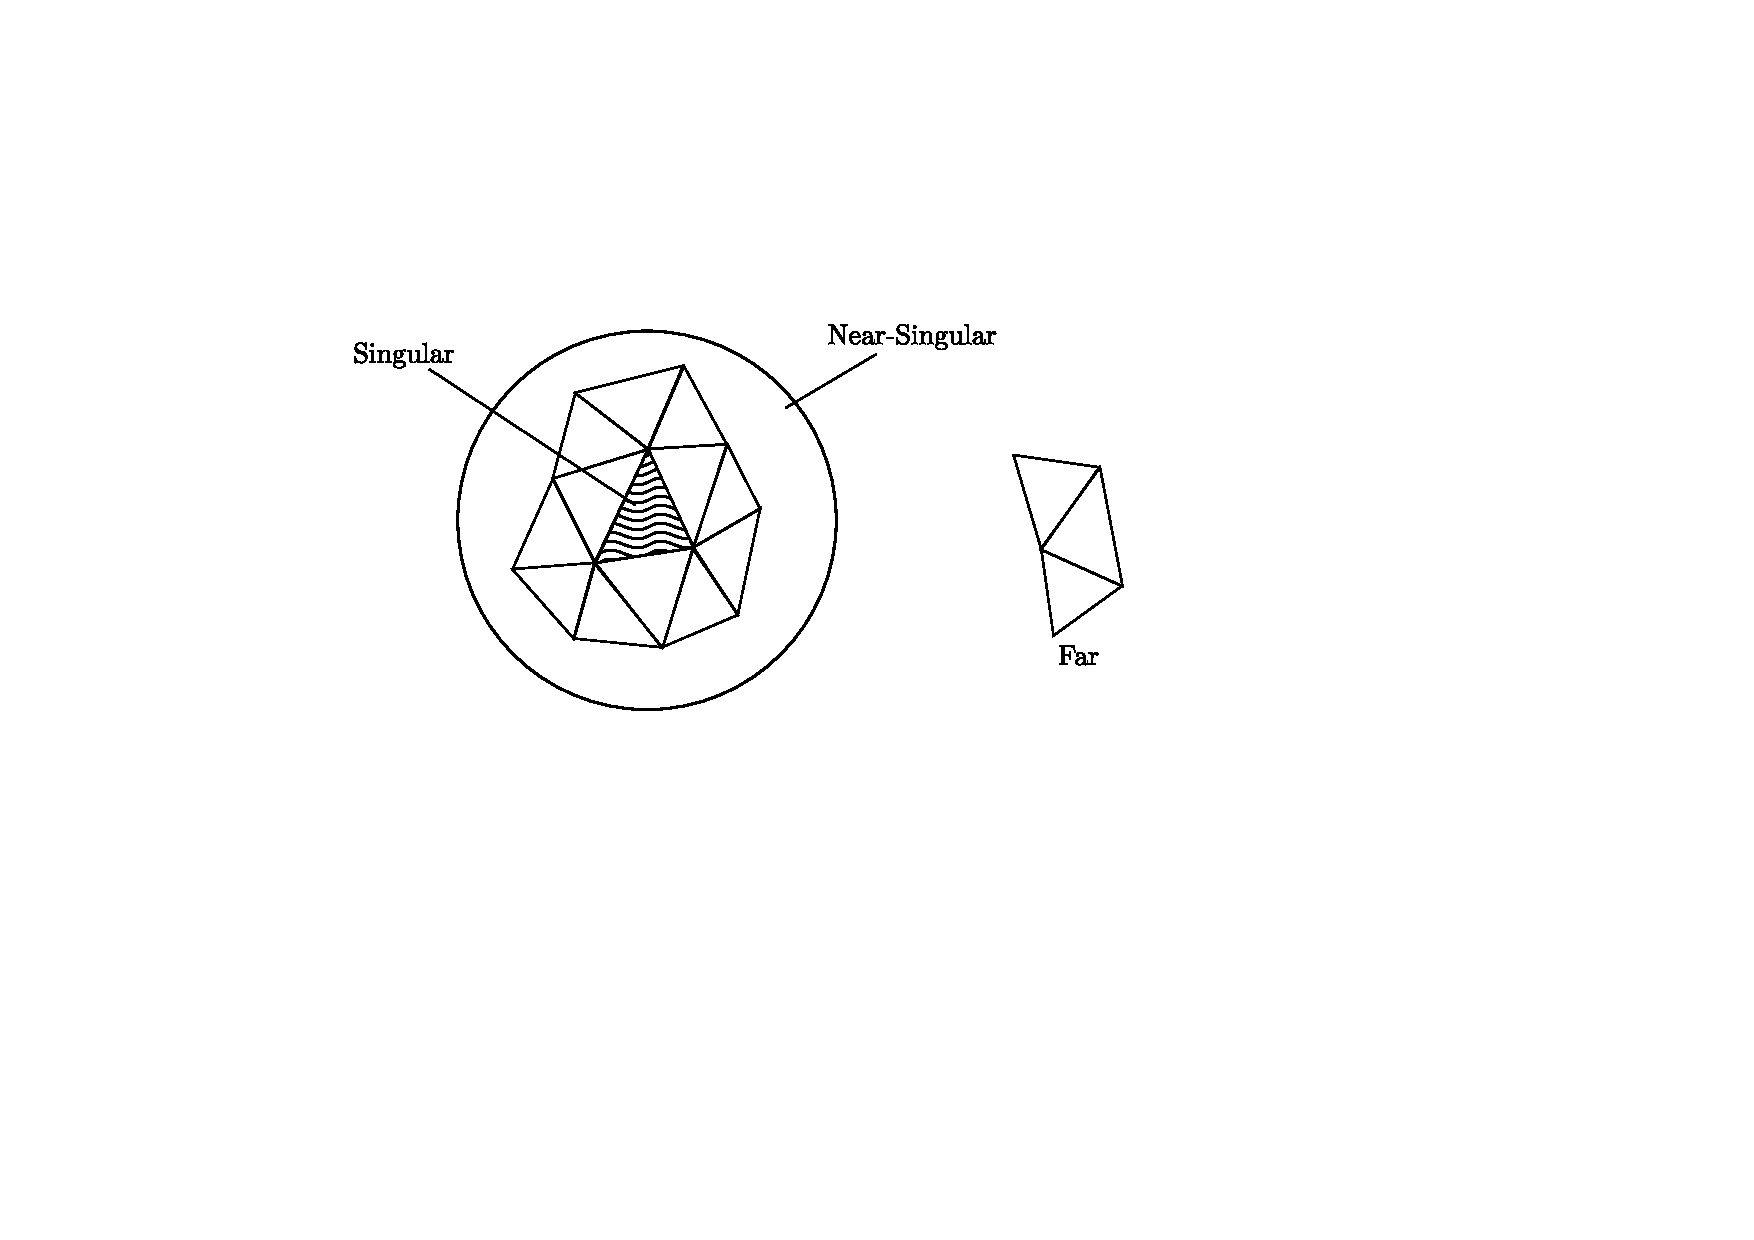
\includegraphics[natwidth=5.15in,natheight=2.6in,width=0.55\textwidth]{IntegrationDomain.pdf}
	\caption{Integration domains}
	\label{fig:integration_domain}
	\end{centering}
\end{figure}
%\clearpage % had to hack this in to get the graphic within the text margins when using the unmodified SIAM class file


Applying Gauss quadrature to the integrals appearing in the coefficients of the boundary element discretization for Laplace's equation, \eqref{eqn:laplace_bem_G} and \eqref{eqn:laplace_bem_dGdn}, for example, gives
%
\begin{eqnarray}
	\int_{\Gamma} G(\vect{x}_i,\vect{x}_j)\;\di{\Gamma_j} & \approx & \sum_{k=1}^{K} q_k\cdot S_j\cdot \frac{1}{|\vect{x}_i-\vect{x}_k|},\;\;\vect{x}_k \in \Gamma_j, \\ 
	\int_{\Gamma} \partiald{G(\vect{x}_i,\vect{x}_j)}{\nhat_j}\;\di{\Gamma_j} & \approx & \sum_{k=1}^{K}q_k\cdot S_j\cdot \frac{d\vect{x}\cdot\nhat_j}{|\vect{x}_i-\vect{x}_k|^{3}},\;\;\vect{x}_k \in \Gamma_j,
\end{eqnarray}

\noindent
with $q_k$ the area-normalized Gauss quadrature weights and $S_j$ the surface area of panel $\Gamma_j$. To control the accuracy of the numerical integration, we vary the number of quadrature points, using for example $K< 4$ for targets that are far from the source panel and $K\sim 20$ for near-singular situations. 
When the target point is on the source panel, the standard approach is to use analytical or semi-analytical methods for the singular and hyper-singular integrals over the panels.
For the Laplace equation, we used a semi-analytical method. 
[[MORE HERE+REF]]
Several analytic integration techniques are at our disposal for dealing with the singular integrals from boundary element methods. Explicit expressions for these integrals over flat triangular domains result in recursive formulae on the edges of the integration triangle. These are available for Laplace potentials \cite{Fata2009} and linear elastic surface potentials \cite{Fata2011}. 
We obtained the analytic integrals for Stokes equation from Fata's formulas for linear elasticity, after setting the Poisson ratio to $1/2$. 

\subsection{Krylov subspace methods}

For large linear systems of equations $A\vect{x}=\vect{b}$, direct solution is generally unfeasible and iterative solution methods are preferred. Krylov subspace methods derive from the Cayley-Hamilton theorem, which states that you can express the inverse of a  matrix $A$ as a linear combination of its powers. A Krylov subspace is spanned by the products of $b$ and powers of $A$; to order-$r$, this is: $K_{r}(A,b) = \text{span}\{ b, Ab, A^{2}b, ..., A^{r-1}b\}$.
Krylov methods include the conjugate gradient method, the biconjugate gradient stabilized method (\textsc{bicgstab}) and the generalized minimal residual method, \gmres \cite{SaadSchultz1986}, which we use. We list the pseudocode of a right-preconditioned {\gmres} algorithm in the Appendix as Algorithm \ref{alg:gmres}. The greatest cost per iteration is the matrix-vector product (matvec), $w\gets A\cdot x$, taking $\O{N^{2}}$ time in a direct implementation. However, given the structure of the coefficient matrix in boundary element methods, this operation can be reduced to $\O{N}$ time using, for example, the fast multiple method.
The key is understanding the matrix-vector product as an $N$-body problem. Let's consider the first-kind integral problem for the Laplace equation. In \eqref{eqn:laplace_matrix} we see that the matrix coefficients are $\int_{\Gamma} G_{ij}\;\di{\Gamma_j}$ in this case. Applying Gauss quadrature to obtain the coefficients 

\subsection{Fast multipole method}

Fast multipole methods were invented to accelerate the solution of $N$-body problems, that is, problems seeking to determine the motion of $N$ bodies that interact with each other via a long-distance effect (like electrostatics or gravitation). A direct approach to such a problem takes $\O{N^{2}}$ time to compute. The first \emph{fast} algorithms for $N$-body problems \cite{Appel1985,BarnesHut1986} combined two ideas: (1) approximating the effect of groups of distant bodies with a few moments (of the charges or masses), and (2) using a hierarchical sub-division of space to determine the acceptable distances to apply these approximations.
 These ideas produced the treecode algorithms, with $\bigO(N\log N)$ time to compute.
The fast multipole method \cite{GreengardRokhlin1987} introduces a third, key idea that leads to $\bigO(N)$ scaling: allowing groups of distant bodies to interact with \emph{groups} of targets, by means of a mathematical representation called local expansion.

A typical $N$-body problem evaluates a potential $\phi$ on $i=1\cdots N$ bodies
using the following expression
%
\begin{equation}\label{eqn:nbody}
	\phi_{i} = \sum_{j=0,\; j\ne i}^{N} m_{j}\cdot\K(\vect{x}_{i},\vect{x}_{j}) \; = \; \sum_{j=0}^{N}\K_{ij}m_{j},
\end{equation}

\noindent where $\K_{i,j} = \K(\vect{x}_{i},\vect{x}_{j})$ is referred to as the \emph{kernel}, and the potential is a solution of an elliptic equation, e.g., the Poisson equation $\vect{F}_i = - \nabla^2 \phi_i$ for gravitation.


%$ RESULTS
\section{Results and discussion}

\subsection{Inexact {\small GMRES} for the solution of Laplace's equation}
To start, we looked at grid-convergence comparing with the analytical solution using a sphere with constant potential and charge on the surface: $\phi = \partialdi{\phi}{\nhat} = 1$. To make surface triangulations of a sphere with increasing refinement, we started with an 8-triangle closed surface, then split recursively each triangle into four smaller ones. Figure \ref{fig:glob_spheres} shows two example discretizations. We solved the boundary-element problem by collocation in both the first-kind and second-kind integral formulations, using a standard right-preconditioned \gmres with fast-multipole-accelerated matrix-vector products and the semi-analytical integrals for the singular terms. For the far-field approximations, we used spherical-harmonic expansions with the following parameters in the \fmm: $\theta_{\text{MAC}} = 0.5$, $p = 10$, and a tolerance of $10^{-6}$ in the iterative solver. 
Figure \ref{fig:laplaceconvergence} shows the resulting convergence for both first-kind and second-kind formulations of the boundary element method on a sphere. They display the expected orders of convergence for boundary element methods: slightly faster than $\O{1/\sqrt{N}}$ in the 1st-kind formulation and $\O{1/N}$ for the 2nd-kind formulation. This gives confidence on our \bem code, the singular/near-singular integral calculations, and the far-field approximation using the \fmm.




\begin{figure}[ht]
\begin{center}
	\subfloat[][128 panels]{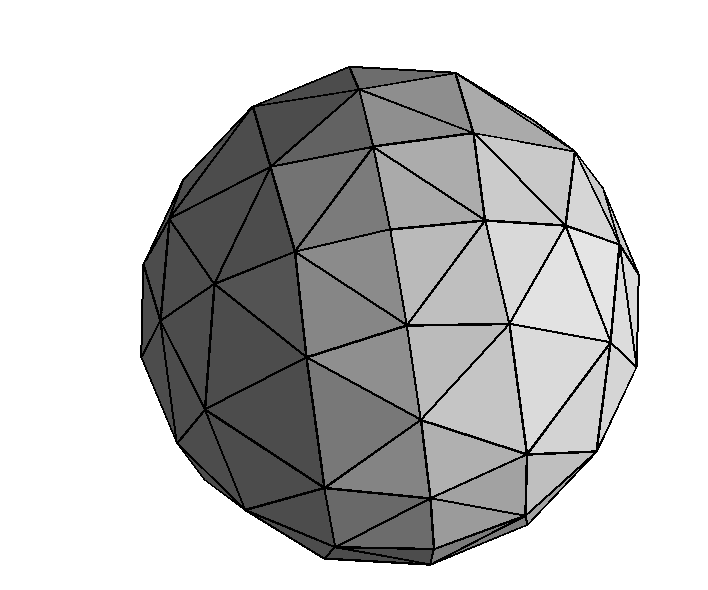
\includegraphics[natwidth=4.73in,natheight=3.94in,width=0.4\textwidth]{sphere128.pdf}\label{fig:sphere128}}\qquad
	\subfloat[][2048 panels]{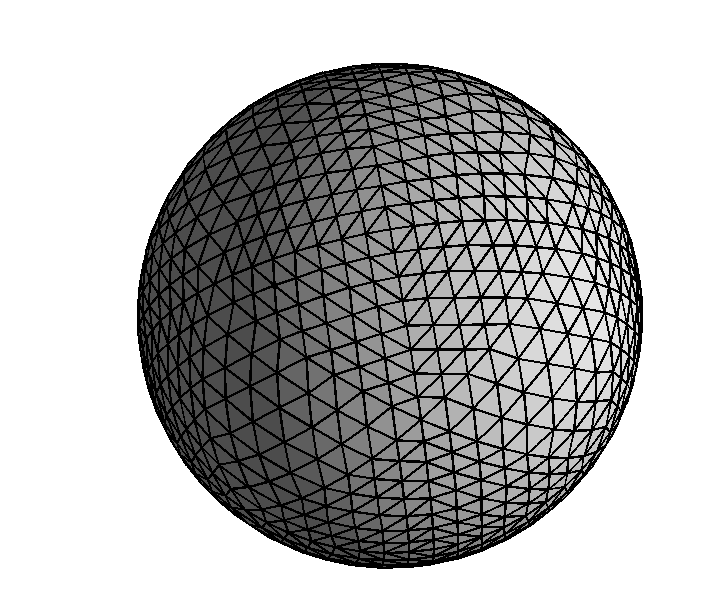
\includegraphics[natwidth=4.73in,natheight=3.94in,width=0.4\textwidth]{sphere2048.pdf}\label{fig:sphere2048}}
	\caption{Triangular discretizations of a spherical surface.}
	\label{fig:glob_spheres}
\end{center}
\end{figure}
%
\begin{figure}[t]
\begin{center}
	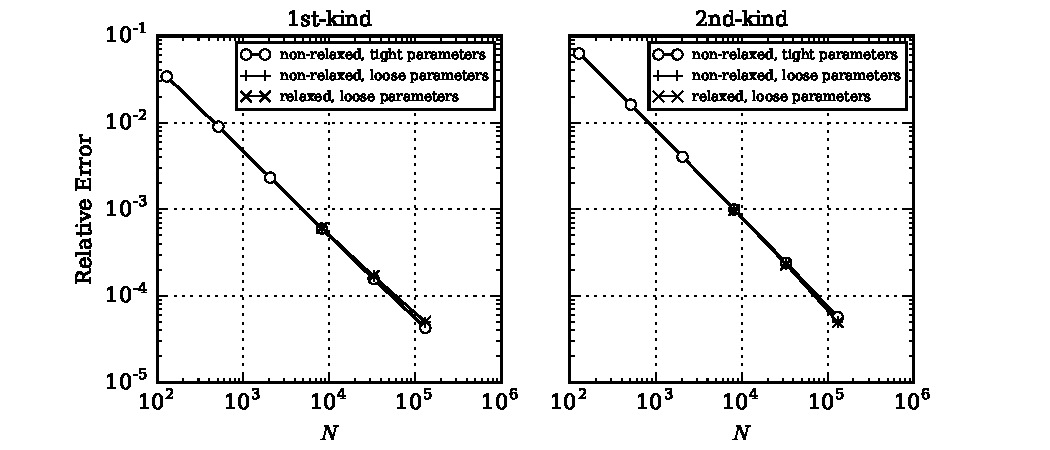
\includegraphics[natwidth=3in,natheight=2in,width=0.5\textwidth]{LaplaceConvergence.pdf}
	\caption{Convergence of 1st-kind (open circles with solid line) and 2nd-kind (open circles with dotted line) solvers for the Laplace equation on a sphere, using a right-preconditioned \gmres with \fmm-accelerated matrix-vecctor products, with parameters: $\theta_{\text{MAC}} = 0.5$, $p=10$, and solver tolerance of $10^{-6}$ (no relaxation).}
	\label{fig:laplaceconvergence}
\end{center}
\end{figure}

Next, we looked at the following test to see how the residual changes as the \gmres iterations proceed and  what value of $p$ is required in the \fmm-accelerated mat-vecs to continue convergence. We discretized a sphere with $32,768$ surface triangles and solved a first-kind integral equation using a solver tolerance of $10^{-5}$ with an initial value of $p$ set to 8. As the residual gets smaller, the value of $p$ needed to maintain convergence of the solver drops, and a low-$p$ of just 3 is sufficient by the seventh iteration. This offers the potential for substantial speed-ups in the calculations, because the translation operators of the \fmm scale from $\bigO(p^{4})$ for spherical harmonics to $\bigO(p^{6})$ for Cartesian expansions.
But we note that only the far-field evaluation can be sped-up with the relaxation strategy, which means that the correct balance between near field and far field in the \fmm could change as we reset $p$ in the later iterations.

\begin{figure}[ht]
	\centering
	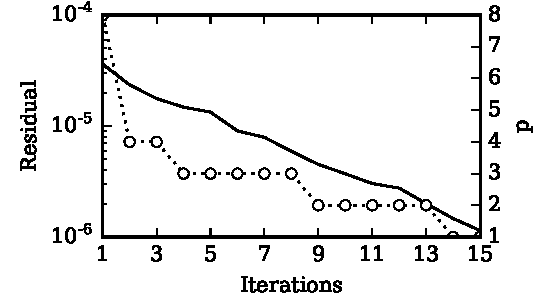
\includegraphics[natwidth=3.7in,natheight=2in,width=0.65\textwidth]{LaplaceResidualIterations.pdf}
	\caption{In a test using a sphere discretized with $32,768$ triangles, the residual $\|r_{k}\|$  (solid line, left axis) decreases with successive \gmres iterations while the necessary $p$ (open circles, right axis) to achieve convergence drops quickly.}
	\label{fig:residualp}
\end{figure}

To find out how much is the potential speed-up, we compared the time to solution for different cases with and without the relaxation strategy. Using three surface discretizations, we solved the boundary-element problem with 1st- and 2nd-kind formulations to a solver tolerance of $10^{-5}$, using a multi-threaded evaluator on 4 \cpu\ cores. In each case, we were careful to set the value of $\ncrit$ to minimize the time to solution of the particular test case. Figure \ref{fig:relaxation_timing} shows the speed-up in the time spent solving the linear system of equations to the specified tolerance. The detailed results are given in the subsequent Tables.


\begin{figure}%[h]
	\centering
	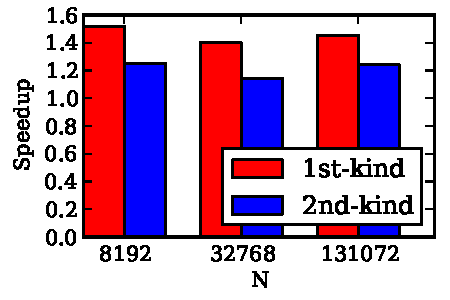
\includegraphics[natwidth=3in,natheight=2in,width=0.45\textwidth]{LaplaceSpeedupRelaxation.pdf}
	\caption{Speedup using a relaxation strategy for three different triangulations of a sphere, using 1st-kind and 2nd-kind integral formulations. (Multi-threaded evaluator running on 4 \cpu\ cores.)}
	\label{fig:relaxation_timing}
\end{figure}


\begin{table}[h]
\footnotesize
\begin{center}
\begin{tabular}{c|cc|cc|c}
  & \multicolumn{2}{c|}{Non-Relaxed} & \multicolumn{2}{c|}{Relaxed} & \\
  N & $\ncrit$ & $\tsolve$ & $\ncrit$ & $\tsolve$ & Speed-up \\
 \hline
   & & & & & \\
  2048 & 400 & 0.27 & 200 & 0.40 & 0.675 \\
  8192 & 400 & 2.58 & 200 & 1.7 & 1.52 \\
  32768  & 400 & 7.1 & 200 & 5.07 & 1.40 \\
  131072  & 400 & 30.1 & 200 & 20.72 & 1.45 \\
 
\end{tabular}
\end{center}
\caption{Speed-ups for the relaxation strategy on a Laplace 1st-kind integral solver, $p=8$, solver tolerance $10^{-5}$.}
\label{tab:laplace_1st_relaxation}
\end{table}%

\begin{table}[h]
\footnotesize
\begin{center}
\begin{tabular}{c|cc|cc|c}
  & \multicolumn{2}{c|}{Non-Relaxed} & \multicolumn{2}{c|}{Relaxed} & \\
  N & $\ncrit$ & $\tsolve$ & $\ncrit$ & $\tsolve$ & Speed-up \\
 \hline
   & & & & & \\
  2048 & 400 & 0.13 & 200 & 0.64 & 0.20 \\
  8192 & 400 & 1.49 & 200 & 1.19 & 1.25 \\
  32768 & 400 & 6.77 & 200 & 5.92 & 1.14 \\
  131072 & 400 & 30.01 & 200 & 24.2 & 1.24 \\
 
\end{tabular}
\end{center}
\caption{Speed-ups for the relaxation strategy on a Laplace 2nd-kind integral solver, $p=8$, solver tolerance  $10^{-5}$.}
\label{tab:laplace_2nd_relaxation}
\end{table}%

The results on Tables \ref{tab:laplace_1st_relaxation} and \ref{tab:laplace_2nd_relaxation} show a speed-up for the three larger grids---also plotted on Figure \ref{fig:relaxation_timing}---of about $1.4\times$ for the 1st-kind integral formulation and $1.2\times$ for the 2nd-kind formulation. These are moderate speedups, but these tests already taught us something: that one has to give up on the idea of partitioning the domain between a near-field and a far-field in a way that balances the time spent computing each one---an accepted idea in \fmm applications. When relaxing the accuracy of the \gmres iterations, the time taken to compute the far field decreases significantly. This means that to minimize time-to-solution when using relaxed \gmres, the near and far fields should not be balanced, but rather the far field should be bloated. As a result, the first couple of iterations are completely dominated by the time to compute the far field, but this is offset by the benefit of much cheaper iterations from then on. This is a simple but unexpected and counter-intuitive algorithmic consequence of the idea of inexact \gmres with \fmm.

It's clear that greater benefits from the relaxation strategy should derive from two situations: (a) where higher accuracy is needed (necessitating an initially higher $p$) , and (b) where the linear system demands a greater number of iterations to reach a set tolerance (resulting in more computations done at low $p$). To demonstrate this, we now present two tests that force these situations. 

\begin{figure}[ht]
	\centering
	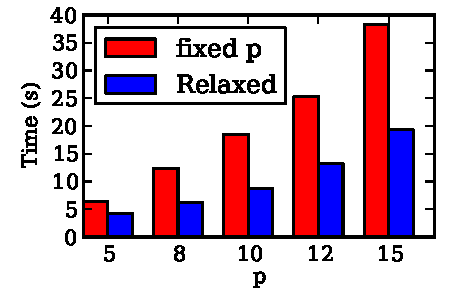
\includegraphics[natwidth=3in,natheight=2in,width=0.45\textwidth]{LaplaceRelaxationP.pdf}
	\caption{Timings for solving a 1st-kind Laplace integral formulation on a sphere discretized with $32,768$ panels, using a relaxed \gmres with different initial values of $p$, compared with a fixed-$p$ solver. The iteration count was capped at 10 for all cases. (Multi-threaded evaluator running on 4 \cpu\ cores.)}
	\label{fig:laplace_p_speedup}
\end{figure}

Figure \ref{fig:laplace_p_speedup} shows the timings obtained in a situation where the initial $p$ is incrementally larger, representing applications that demand higher accuracy. The test consists of a 1st-kind Laplace integral solver on a sphere discretized with $32,768$ panels, enforcing a fixed number of $10$ \gmres iterations (which results in a residual of $~5.5\times 10^{-5}$ for the sphere). Table \ref{tab:laplace_1st_p_relaxation} shows the data for this test: the speed-up is greater with larger initial values of $p$, leveling at around $2\times$ when initial $p$ is greater than 8. Note again that the shortest time-to-solution requires an unbalanced tree on the first iteration, with a bloated far field. This means that the first (high-$p$) iteration is much slower than the corresponding fixed-$p$ case: the speed-up is thus purely a product of the low-cost later iterations.

\begin{table}[h]
\footnotesize
\begin{center}
\begin{tabular}{c|cc|cc|c}
  & \multicolumn{2}{c|}{Relaxed} & \multicolumn{2}{c|}{Non-Relaxed} & \\
  $p$ & $\ncrit$ & $\tsolve$ & $\ncrit$ & $\tsolve$ & Speedup \\
   \hline
   & & & & & \\
  5 & 100 & 4.21 & 100 & 6.34 & 1.51 \\
  8 & 100 & 6.24 & 400 & 12.4 & 1.99 \\
  10 & 150 & 8.76 & 400 & 18.5 & 2.11 \\
  12 & 150 & 13.2  & 600 & 25.3 & 1.92 \\
  15 & 150 & 19.3 & 600 & 38.3 & 1.98 \\
 
\end{tabular}
\end{center}
\caption{Speed-up when using a relaxation strategy on a Laplace 1st-kind integral solver, compared with a non-relaxed solver, with increasing value of the initial $p$ (representing increased accuracy demands of the application), for a sphere discretized with $32,768$ panels. (Multi-threaded evaluator running on 4 \cpu\ cores.)}
\label{tab:laplace_1st_p_relaxation}
\end{table}%

The final case looks at the situation where the application might demand large iteration counts, as could be encountered in harder-to-precondition cases. Keeping the value of $p$ fixed at 10, we ran several cases with increasing number of (set) \gmres iterations, representing more ill-conditioned problems. Figure \ref{fig:laplace_iterations_speedup} shows how cases with larger iteration counts experience greater speed-up from the relaxation strategy. As seen in the data of Table \ref{tab:laplace_1st_iterations_relaxation}, each non-relaxed iteration adds approximately $1.68$s to $\tsolve$, while each relaxed iteration adds $0.276$s; we can thus extrapolate a speed-up nearing $5\times$ at 100 iterations.



\begin{figure}[ht]
	\centering
	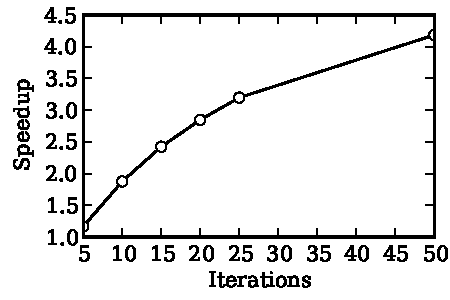
\includegraphics[natwidth=3in,natheight=2in,width=0.5\textwidth]{LaplaceRelationIterations.pdf}
	\caption{Speed-ups for solving a 1st-kind Laplace integral problem on a sphere discretized with $32,768$ panels, as the \gmres iteration count increases; $p=10$ for all cases. (Multi-threaded evaluator running on 4 \cpu\ cores.)}
	\label{fig:laplace_iterations_speedup}
\end{figure}


\begin{table}[h]
\footnotesize
\begin{center}
\begin{tabular}{c|cc|cc|c}
  & \multicolumn{2}{c|}{Relaxed} & \multicolumn{2}{c|}{Non-Relaxed} & \\
  Iterations & $\ncrit$ & $\tsolve$ & $\ncrit$ & $\tsolve$ & Speedup \\
 \hline
   & & & & & \\
  5 & 100 & 8.57 & 400 & 10.0 & 1.17 \\
  10 & 100 & 9.81 & 400 & 18.4 & 1.88 \\
  15 & 100 & 11.1 & 400 & 26.9 & 2.42 \\
  20 & 100 & 12.4 & 400 & 35.3 & 2.85 \\
  25 & 100 & 13.7 & 400 & 43.8 & 3.20 \\
  50 & 100 & 20.6 & 400 & 86.2 & 4.18 \\
 
\end{tabular}
\end{center}
\caption{Speed-up of the relaxation strategy on solving a Laplace 1st-kind integral problem on a sphere discretized with $32,768$ panels, with increasing iteration count; $p$ fixed to a value of 10. (Multi-threaded evaluator running on 4 \cpu\ cores.)}
\label{tab:laplace_1st_iterations_relaxation}
\end{table}%

\subsection{Inexact {\small GMRES} for solving the Stokes equation}
Like before, we start with a grid-convergence study to build confidence that the Stokes solver is correct and converges to the right solution at the expected rate. As an application of the Stokes equation, we chose low-Reynolds-number flow, using a spherical geometry for the grid-convergence study. This classical problem of fluid mechanics has an analytical solution that gives the drag force on the sphere as $F_d = 6\pi\mu Ru_x$, where $\mu$ is the viscosity of the fluid, $R$ is the Reynolds number and $u_x$ is the free stream velocity, taken in the $x$-direction. We solve a first-kind integral equation for the traction force, $\vect{t}$, by imposing $\vect{u} = (1,0,0)^{T}$ at the center of every panel, and compute the drag force with

\begin{equation}
	\label{eqn:stokes_traction_drag}
	F_d = \int_\Gamma t_x\;\di{\Gamma'} = \sum_{j=1}^{N} t_{x_j}\cdot A_j
\end{equation}

For all the tests, we set $R=1$, $u_x = 1$ and $\mu = 10^{-3}$, giving a drag force of $F_d = 0.01885$. We solve the integral problem using a boundary element method with fast-multipole-accelerated mat-vecs in a \gmres solver. We first increased the value of $p$ until the solution stopped improving, and settle for $p=16$ in this case, using a $10^{-5}$ tolerance in the iterative solver.
Figure \ref{fig:stokes_convergence} shows that we indeed observe convergence at the expected rate of $\O{1 / \sqrt{N}}$, for first-kind integral equations.

\begin{figure}[ht]
\begin{center}
	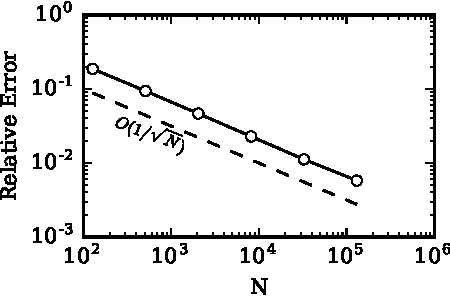
\includegraphics[natwidth=3in,natheight=2in,width=0.5\textwidth]{StokesConvergence.pdf}
	\caption{Convergence of the boundary-integral solution for Stokes flow around a sphere, using a  first-kind equation; $p=16$, linear system solved to $10^{-5}$ tolerance.}
	\label{fig:stokes_convergence}
\end{center}
\end{figure}

Like with the Laplace equation, we need to show that the relaxation strategy does not hinder convergence and that there is a potential for speed-ups. We solved the problem of Stokes flow around a sphere, discretized with $8,192$ panels, and compared the residual history of a fixed-$p$ solver with a relaxed \gmres with an initial $p=16$. Figure \ref{fig:stokes_residual_history_relaxed} shows that the residual history (for the traction force) is similar for both relaxed and non-relaxed \gmres, both methods reaching the stipulated tolerance of $10^{-5}$ after about 27 iterations.
The number of iterations needed to converge is larger in the case of the Stokes equation compared to the Laplace equation, which bodes well for the speed-up that we could get from relaxation. Moreover, the fast multipole expansions for the Stokes kernel are equivalent to four Laplace expansions, which combines with the larger number of iterations to offer greater speed-ups.


\begin{figure}%[t]
\begin{center}
	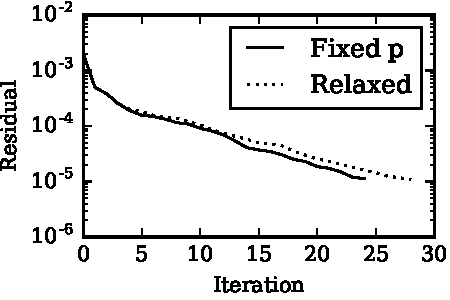
\includegraphics[natwidth=3in,natheight=2in,width=0.5\textwidth]{StokesResidualHistory.pdf}
	\caption{Residual history solving for surface traction on the surface of a sphere (first-kind integral problem), with a $10^{-5}$ solver tolerance, $8,192$ panels, and $p=16$ in the multipole expansions.}
	\label{fig:stokes_residual_history_relaxed}
\end{center}
\end{figure}

Figure \ref{fig:stokes_relaxation_breakdown} illustrates clearly how we need to adjust the balance between near field and far field when using relaxation strategies. Because most of the time is spent computing at the low values of $p$, we need to start with a bloated far field. The bar plot shows the breakdown of time spent in the {\ptop} and {\mtol} kernels for each iteration: although the first iteration is unbalanced, with far field taking about 8 times as much \cpu\ time as near field, later iterations are close to balanced and the total time to solution is optimal. 
The figure also includes a plot of the residual history. We should add that we ran extensive tests on the minimum value of $p$ that could be allowed in the relaxed solver, without degrading convergence and accuracy. Table \ref{tab:stokes_min_p} presents some of the data from these tests: for finer surface discretizations, the error degrades when the relaxed value of $p$ is allowed to drop below 3 or 4. To be conservative and avoid any degradation in accuracy, we used a $\pmin=5$ for all further cases with the Stokes equation.


\begin{figure}%[ht]
\begin{center}
	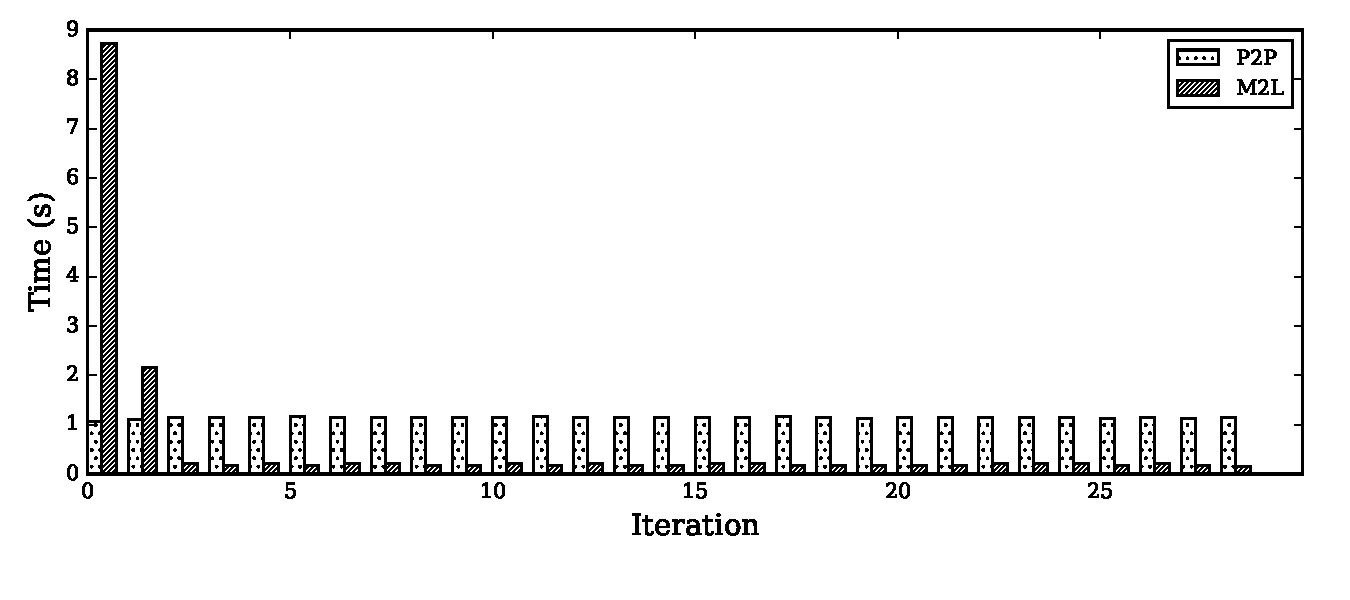
\includegraphics[natwidth=3in,natheight=2in,width=0.5\textwidth]{StokesSolveBreakdown.pdf}
	\caption{Residual history solving for surface traction on the surface of a sphere, with time breakdown between {\ptop} and {\mtol}. $10^{-5}$ solver tolerance, $8,192$ panels, $p=16$.}
	\label{fig:stokes_relaxation_breakdown}
\end{center}
\end{figure}



\begin{table}[ht]
\footnotesize
\begin{center}
\begin{tabular}{c|cc|cc|cc}
  & \multicolumn{2}{c|}{2048 panels} & \multicolumn{2}{c|}{8192 panels} & \multicolumn{2}{c}{32768 panels} \\
 $\pmin$ & Error & $it$ & Error & $it$ & Error & $it$ \\ \hline
  & & & & & & \\
 5 & $4.70\times 10^{-2}$ & 22 & $2.44\times 10^{-2}$ & 28 & $1.34\times 10^{-2}$ & 28 \\
 4 & $4.49\times 10^{-2}$ & 23 & $2.51\times 10^{-2}$ & 29 & $1.25\times 10^{-2}$ & 29 \\
 3 & $4.64\times 10^{-2}$ & 22 & $2.78\times 10^{-2}$ & 29 & $1.39\times 10^{-2}$ & 29 \\
 2 & $4.95\times 10^{-2}$ & 25 & $2.62\times 10^{-2}$ & 33 & $3.18\times 10^{-2}$ & 39 \\
 1 & $4.96\times 10^{-2}$ & 25 & $2.99\times 10^{-2}$ & 51 & $4.77\times 10^{-2}$ & 53 
\end{tabular}
\end{center}
\caption{Effect of $p_{\text{min}}$ on accuracy and convergence for Stokes flow around a sphere for differing values of $N$. Error is on the total drag force in the $x$-direction, $F_x$.}
\label{tab:stokes_min_p}
\end{table}%

Figure \ref{fig:stokes_speedup} shows the speed-up resulting from the relaxed \gmres iterations for four, increasingly finer surface discretizations. For $N=8,192$ and above, speed-up is $3.5\times$ or more.


\begin{figure}[ht]
\begin{center}
	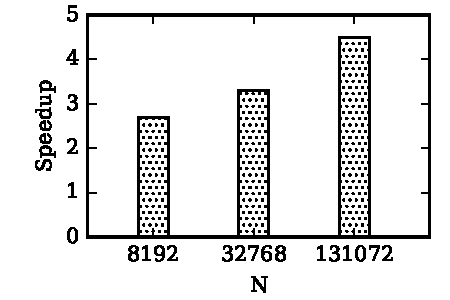
\includegraphics[natwidth=3in,natheight=2in,width=0.5\textwidth]{StokesSpeedupRelaxation.pdf}
	\caption{Speed-up for solving first-kind Stokes equation on the surface of a sphere, varying $N$. $10^{-5}$ solver tolerance, $p=16$. }
	\label{fig:stokes_speedup}
\end{center}
\end{figure}

\subsection{Application to red blood cells in Stokes flow}

A number of medical applications will benefit from greater understanding of the microflows around red blood cells and of the mechanical effects on the cells from this flow. 
The most notable example is perhaps the deadly malaria infection, which changes red blood cells making them stiffer thus disrupting the flow of blood in capillaries \cite{FedosovETal2011}.
Any design of a biomedical device that processes blood at the micrometer-scale needs to consider the mechanical behavior of blood at the cellular level \cite{Freund2014}. Blood is a dense suspension of mostly red blood cells and smaller concentrations of white blood cells and platelets. The flow regime in small capillaries is at very low Reynolds numbers, and thus completely dominated by viscous effects. 
Red blood cells are very flexible, so any physiologically realistic simulation should take into account their elastic deformations. But here we are only attempting to show the benefit of our relaxation strategy on the Stokes solver, and thus limit our study to the steady Stokes flow around a red-blood-cell geometry. The unsteady problem of coupled Stokes flow and linear elasticity can be approached by repeated solution of boundary-integral problems at every time step, and would equally benefit from the speed-ups seen on a single Stokes solution.

To create a surface discretization for a red blood cell, we start with a sphere discretized into triangular panels and transform every vertex $v = v(x,y,z)$, with $x,y,z\in [-1,1]$, into $v' = v'(x',y',z(\rho'))$ using the formula presented in Ref.~\cite{EvansFung1972}:
%
\begin{equation}
	\label{eqn:rbc_parameterization}
	z(\rho) = \pm \frac{1}{2}\sqrt{1 - \left(\frac{\rho}{r}\right)^{2}}\left ( C_0 + C_2 \left(\frac{\rho}{r}\right)^{2} + C_4\left(\frac{\rho}{r}\right)^{4}\right ),
\end{equation}

\noindent where $x' = x\cdot r,\; y' = y\cdot r,\; \rho = \sqrt{x'^{2}+y'^{2}}$, and the coefficients are: $r=3.91\mu$m,  $C_0= 0.81\mu$m, $C_2= 7.83\mu$m and $C_4=-4.39\mu$m.
Figure \ref{fig:glob_rbc} shows two examples of transformed shapes obtained from sphere triangulations using Equation \eqref{eqn:rbc_parameterization}.

% This figure behaved weird when using the unmodified SIAM class file, and the images appeared displaced upwards; needed to hack it with \vspace{1cm} before each \subfloat
% It now works well with the RequirePackage lines commented out on the .cls file !!
\begin{figure}[ht]
\begin{center}
	\subfloat[512 panels]{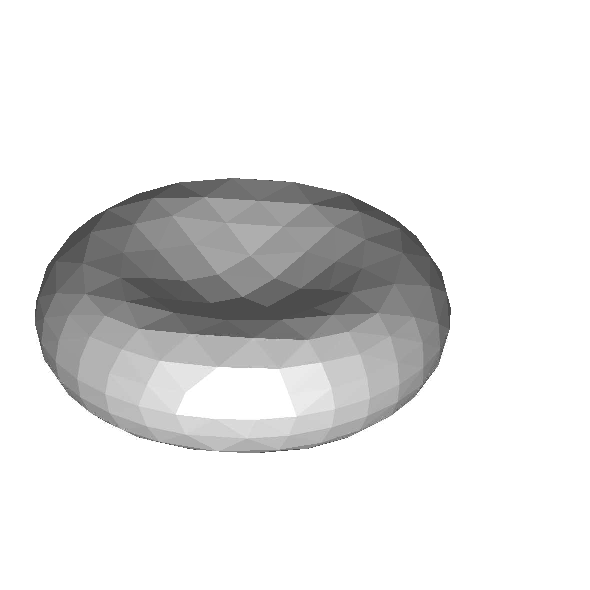
\includegraphics[natwidth=2.94in,natheight=1.94in,width=0.3\textwidth]{RBC512.pdf}\label{fig:rbc512}}\qquad
	\subfloat[2048 panels]{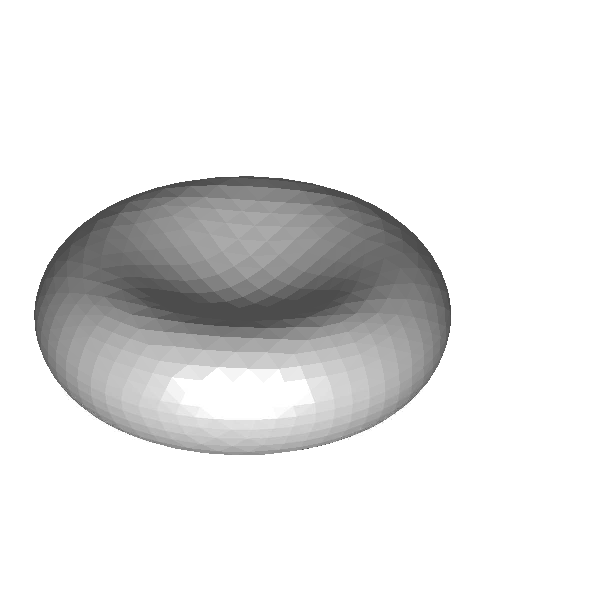
\includegraphics[natwidth=2.94in,natheight=1.94in,width=0.3\textwidth]{RBC2048.pdf}\label{fig:rbc2048}}
	\caption{Surface geometries of red blood cells obtained from transforming sphere triangulations using Equation \eqref{eqn:rbc_parameterization}.}
	\label{fig:glob_rbc}
\end{center}
\end{figure}

A grid-convergence study using the geometry of a red blood cell requires that we use Richardson extrapolation \cite{roache1998}, since we don't have an analytical solution for this situation. We calculated the drag on a red blood cell in uniform Stokes flow using three surface meshes, consecutively refined by a constant factor $c=4$. 
If the value $f_1$ corresponds to that obtained using the coarsest mesh and $f_2$ and $f_3$ to those using consecutively refined ones, then we can obtain the extrapolated value approximating the exact solution with the following formula:

\begin{equation}
	\bar{f} = \frac{f_1f_3-f_2^{2}}{f-1 -2f_2+f_3}
\end{equation}

Table \ref{tab:rbc_richardson_values} presents the computed values of the drag force obtained with three different meshes, of sizes $N=512$, $2048$ and $8192$. We can also obtain the \emph{observed order of convergence}, $p$, as follows
%
\begin{equation}
	p = \frac{\ln{\left(\frac{f_2-f_1}{f_3-f_2}\right)}}{\ln{c}},
\end{equation}

\noindent where $c$ is the refinement ratio between two consecutive meshes. With the values in Table \ref{tab:rbc_richardson_values}, the observed order of convergence comes out at $0.481$, matching our expected rate of convergence of $\O{\sqrt{N}}$. 
Figure \ref{fig:rbc_extrapolated_convergence} shows a plot of the error with respect to the extrapolated value, as a function of the mesh size. The plot includes the error obtained with four meshes, with the extrapolated value obtained with the first three, coarser meshes.

\begin{table}[h]
\footnotesize
\begin{center}
\begin{tabular}{c|c}
	$N$ & $f_x$ \\
	\hline
	& \\
	$512$ & $-0.059$ \\
	$2048$ & $-0.071$ \\ 
	$8192$ & $-0.077$ \\
%	$32768$ & $-0.080$
\end{tabular}
\end{center}
\caption{Surface mesh sizes and calculated drag force for the convergence study using a red blood cell in uniform Stokes flow.}
\label{tab:rbc_richardson_values}
\end{table}%


\begin{figure}
\begin{center}
	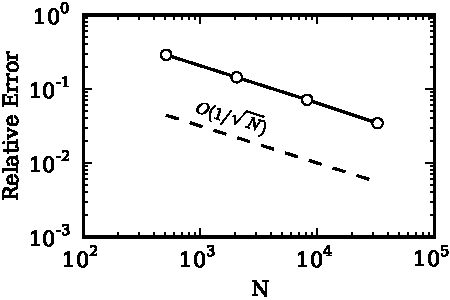
\includegraphics[natwidth=3in,natheight=2in,width=0.5\textwidth]{EthrocyteConvergence.pdf}
	\caption{Observed convergence for Stokes flow around red blood cells, with respect to the extrapolated value of the drag coefficient, using Richardson extrapolation \cite{roache1998}.}
	\label{fig:rbc_extrapolated_convergence}
\end{center}
\end{figure}


The calculations with increasingly finer surface meshes take more time to complete not only because the number of unknowns is larger, but also because they may require a greater number of iterations to converge to a desired residual.
Figure \ref{fig:single_cell_iterations} shows that the number of iterations needed as the surface mesh varies from size $N=128$ to $8,192$ increases from 19 to 37. For further refined meshes, the number of iterations remains about the same. This is an indication that the surface mesh is sufficiently refined with $8,192$ panels for one red blood cell.

\begin{figure}
\begin{center}
	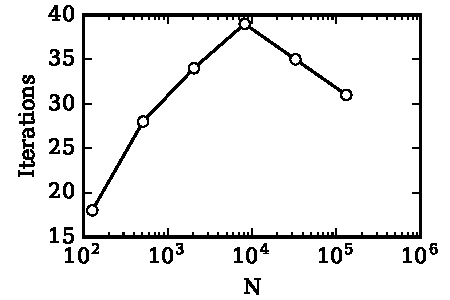
\includegraphics[natwidth=3in,natheight=2in,width=0.5\textwidth]{EthrocyteSingleCellIterations.pdf}
	\caption{Number of iterations needed for the system to converge for increasingly refined surface meshes on one red blood cell; $p = 16$, target residual $10^{-5}$.}
	\label{fig:single_cell_iterations}
\end{center}
\end{figure}


For the next tests, we used several red blood cells in a sparse spatial arrangement. Realistic blood flows have densely packed red blood cells, but the purpose of this test is to simply demonstrate the boundary element solver with a larger problem. We set up a collection of red blood cells by making copies of a discretized cell, then randomly rotating each one, and shifting it spatially in each  coordinate direction by a positive random amount that ensures they do not overlap. The resulting arrangement may look like that shown in Figure \ref{fig:multiple_cells}.

% This figure behaved weird with the unmodified SIAM class file, and the images appeared displaced upwards, needing to hacked it with \vspace{1.2cm} before \includegraphics
% Now it works well with the modified SIAM class file
\begin{figure}[ht]
\begin{center}
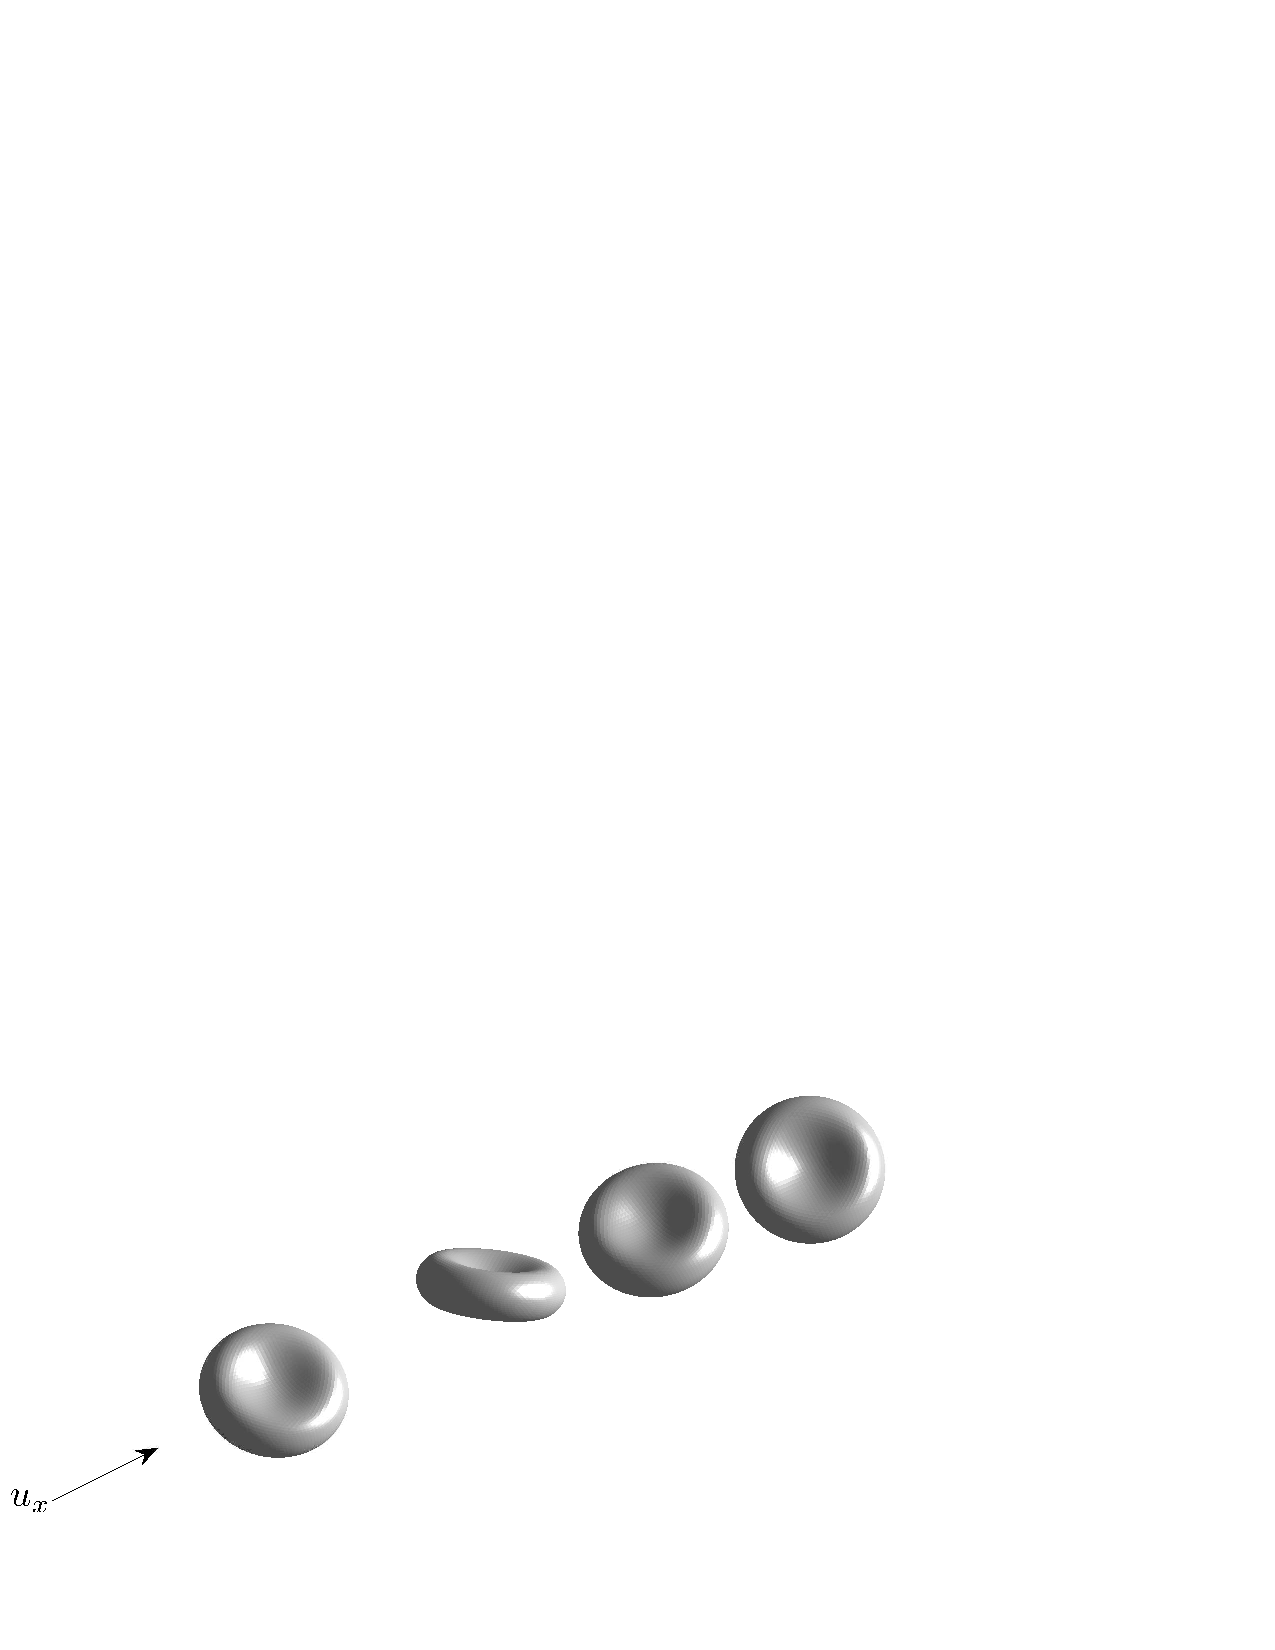
\includegraphics[natwidth=6in,natheight=2.88in,width=0.75\textwidth]{4Cells_arrow.pdf}
	\caption{Surfaces for four red blood cells in a uniform Stokes flow.}
	\label{fig:multiple_cells}
\end{center}
\end{figure}

Using 2, 4 and 8 red blood cells, we looked at the number of iterations needed to converge to a solver tolerance of $10^{-5}$ when using three different surface mesh sizes on each cell: $N=2048$, $8192$ and $32,768$. In all cases $p = 16,\;p_{\text{min}} = 5$. Figure \ref{fig:multiple_cell_iterations} shows that the number of iterations needed to converge increases sharply with the number of red blood cells in the system, while the number of panels per cell has a smaller effect in this range of mesh sizes. In all cases, the number of iterations is between 45 and 65, and thus we expect to see good speed-ups using the relaxation strategy.



\begin{figure}
\begin{center}
	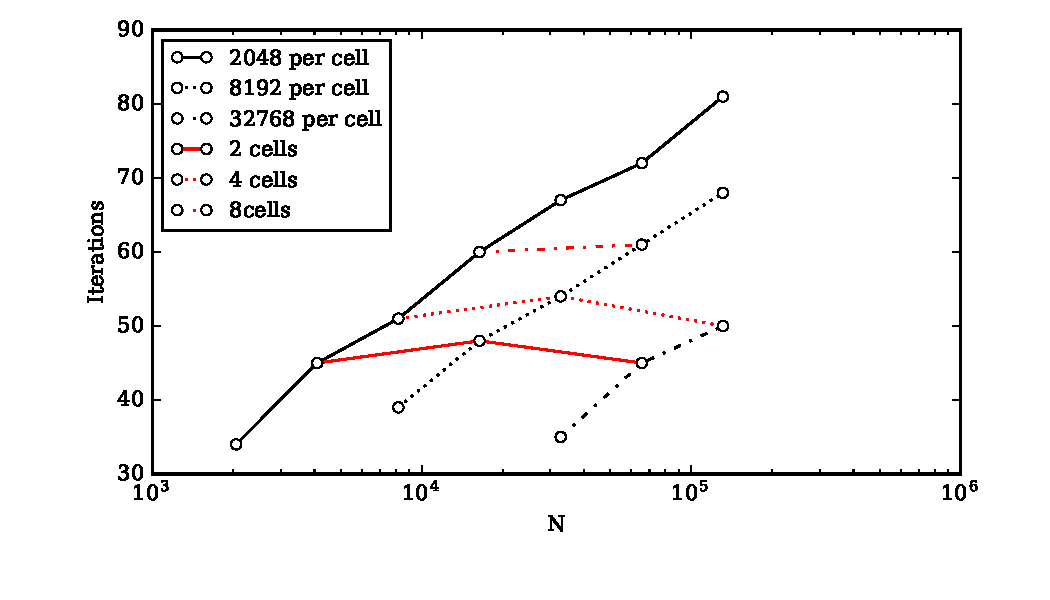
\includegraphics[natwidth=7in,natheight=3.5in,width=0.85\textwidth]{EthrocyteMultipleCellIterations.pdf}
	\caption{Number of iterations needed to converge to a desired residual of $10^{-5}$ for systems with multiple red blood cells, discretized with different mesh sizes ($p = 16$).}
	\label{fig:multiple_cell_iterations}
\end{center}
\end{figure}

We completed several tests of the relaxation strategy, using between 1 and 64 red blood cells, and various mesh sizes on each cell. The common parameter settings for these tests are listed in Table \ref{tab:cells_relaxation_settings} and, in each case, we chose the value of $\ncrit$ (establishing the balance between near and far field) to obtain the smallest time to solution for that run. The detailed results are listed in Tables \ref{tab:single_cell_relaxation_results}, \ref{tab:multiple_cell_relaxation_results_2048}, \ref{tab:multiple_cell_relaxation_results_8192} and \ref{tab:multiple_cell_relaxation_results_32768}, and Figure \ref{fig:multiple_cell_speedup} shows a summary of the observed speed-ups, mostly hovering close to $4\times$. The largest problems, with a total of $131,072$ panels (all cells combined), are atypical because in these cases we are unable to use the efficient sparse-matrix representation of the near field, due to the large memory requirement. But this can also be seen as an advantage of the relaxation strategy, which leads to using smaller near fields and thus extends the range of problem sizes where we can use the efficient sparse-matrix representation. Indeed, if one needed to solve a problem of size $N=131,072$ (on one \cpu\ using four threads, like we do here), then the potential for a $7\times$ speed-up is real.

\begin{table}[h]
\footnotesize
\begin{center}
\begin{tabular}{c|c}
 Variable & Setting \\ 
\hline
 & \\
 $p_{\text{initial}}$ & $16$ \\
 $p_{\text{min}}$ &  $5$ \\
 solver tolerance & $10^{-5}$ \\
 Near-field & Sparse matrix \\
 Threads & $4$ \\
 Solver & {\gmres} \\ 
 Preconditioner & None
\end{tabular}
\end{center}
\caption{Parameters for the tests of the relaxation strategy with red blood cells in uniform Stokes flow.}
\label{tab:cells_relaxation_settings}
\end{table}%


\begin{table}[htdp]
\footnotesize
\begin{center}
\begin{tabular}{c|c|c|c|c|c|c}
 & & \multicolumn{2}{c|}{Non-relaxed} & \multicolumn{2}{c|}{Relaxed} \\
 & & \multicolumn{2}{c|}{} & \multicolumn{2}{c|}{} \\
 N & \# unknowns & $\ncrit$ & $t_{\text{solve}}$ & $\ncrit$ & $t_{\text{solve}}$ & Speedup \\\hline
 & & & & & \\
 2048 & 6144 & 200 & 44.5 & 100 & 11.0 & 4.05 \\
 8192 & 24576 & 400 & 177 & 150 & 52.4 & 3.37 \\
 32768 & 98304 & 400 & 848 & 150 & 223 & 3.80 \\
 131072 & 393216 & 600 & 6386\footnotemark[1] & 150 & 874 & 7.31\footnotemark[1] \\	
\end{tabular}
\end{center}
\caption{Timings and speed-up of the relaxation strategy on a single red blood cell in uniform Stokes flow, with the test parameters shown in Table \ref{tab:cells_relaxation_settings}.}
\label{tab:single_cell_relaxation_results}
\end{table}%

\footnotetext[1]{Due to memory restrictions, the sparse-matrix representation of the near-field could not be used, resulting in a much slower {\ptop} evaluation.}


\begin{table}[htdp]
\footnotesize
\begin{center}
\begin{tabular}{c|c|c|cc|cc|c}
\multicolumn{8}{c}{2048 panels / cell} \\
& & & \multicolumn{2}{c}{Non-relaxed} & \multicolumn{2}{c}{Relaxed}\\
N & \# unknowns & $N_c$ & $\ncrit$ & $\tsolve$ & $\ncrit$ & $\tsolve$ & Speedup \\ \hline
& & & & & & &  \\
2048 & 6144 & 1 & 200 & 44.5 & 100 & 11.0 & 4.05 \\ 
8192 & 24576 & 4 & 200 & 236 & 150 & 59.8 & 3.95 \\ 
32768 & 98304 & 16 & 400 & 1261 & 150 & 331 & 3.81 \\
131072 & 393216 & 64 & 300 & 9982\footnotemark[1] & 100 & 1606 & 6.22\footnotemark[1] \\
\end{tabular}
\end{center}
\caption{Timings and speed-up of the relaxation strategy with several red blood cells in uniform Stokes flow, each cell discretized with 2048 panels and test parameters shown in Table \ref{tab:cells_relaxation_settings}.}
\label{tab:multiple_cell_relaxation_results_2048}
\end{table}


\begin{table}[htdp]
\footnotesize
\begin{center}
\begin{tabular}{c|c|c|cc|cc|c}
\multicolumn{8}{c}{8192 panels / cell} \\
& & &  \multicolumn{2}{c}{Non-relaxed} & \multicolumn{2}{c}{Relaxed}\\
N & \# unknowns & $N_c$ & $\ncrit$ & $\tsolve$ & $\ncrit$ & $\tsolve$ & speedup \\ \hline
& & & & & & &  \\
8192 & 24576 & 1 & 400 & 177 & 150 & 52.4 & 3.37 \\ 
32768 & 98304 & 4 & 400 & 1375 & 150 & 315 & 4.37 \\
131072 & 393216 & 16 & 300 & 15980\footnotemark[1] & 100 & 1692 & 9.44\footnotemark[1] \\
\end{tabular}
\end{center}
\caption{Timings and speed-up of the relaxation strategy with several red blood cells in uniform Stokes flow, each cell discretized with $8,192$ panels and test parameters shown in Table \ref{tab:cells_relaxation_settings}.}
\label{tab:multiple_cell_relaxation_results_8192}
\end{table}


\begin{table}[htdp]
\footnotesize
\begin{center}
\begin{tabular}{c|c|c|cc|cc|c}
\multicolumn{8}{c}{32768 panels / cell} \\
& & & \multicolumn{2}{c}{Non-relaxed} & \multicolumn{2}{c}{Relaxed}\\
N & \# unknowns & $N_c$ & $\ncrit$ & $\tsolve$ & $\ncrit$ & $\tsolve$ & speedup \\ \hline
& & & & & & &  \\
32768 & 98304 & 1 & 400 & 848 & 150 & 223 & 3.80 \\
131072 & 393216 & 4 & 300 & 9629\footnotemark[1] & 100 & 1247 & 7.72\footnotemark[1] \\	
\end{tabular}
\end{center}
\caption{Timings and speed-up of the relaxation strategy with several red blood cells in uniform Stokes flow, each cell discretized with $32,768$ panels and test parameters shown in Table \ref{tab:cells_relaxation_settings}.}
\label{tab:multiple_cell_relaxation_results_32768}
\end{table}


\begin{figure}[ht]
\begin{center}
	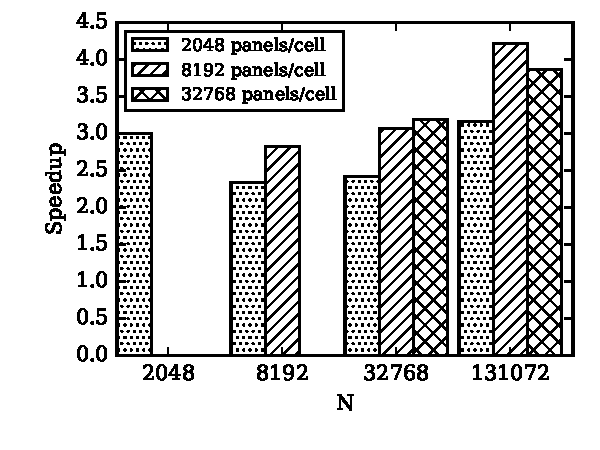
\includegraphics[natwidth=4in,natheight=3in,width=0.55\textwidth]{EthrocyteMultipleCellSpeedup.pdf}
	\caption{Speed-ups of the relaxation strategy with several red blood cells in uniform Stokes flow, using different mesh sizes on each cell. The abscissa value corresponds to the total number of panels (all cells). Test parameters shown in Table \ref{tab:cells_relaxation_settings}.}
	\label{fig:multiple_cell_speedup}
\end{center}
\end{figure}




\section{Conclusion} 

We have shown the first successful application of a relaxation strategy for fast-multipole-accelerated boundary element methods, based on the theory of inexact \gmres. Testing the relaxation strategy on Laplace problems, we confirmed that it converges to the right solution, it provides moderate speed-ups over using a fixed $p$, and it leads to initially bloated far-fields to obtain the minimum time to solution.
Exploring the performance advantage of relaxing the value of $p$ as \gmres iterations advance, we concluded that problems requiring high accuracy and/or resulting in more ill-conditioned linear systems will experience the best speed-ups, which for Laplace problems can be in the order of $2-4\times$.

In the case of the Stokes equation, the speed-ups that can be obtained using a relaxation strategy are larger, due to the fact that Stokes problems require both more iterations to converge (and the relaxed solver spends more time at low $p$) and more work per iteration (equivalent to four Laplace evaluations). Relaxed \gmres iterations in this case reduced the time to solution by $3.5\times$ to $4.5\times$. We found that it's important for Stokes problems to also enforce a minimum value of $p$ to avoid accuracy or convergence degradation.


\Appendix
\section{Algorithm listings}\label{sec:algorithms}
 
 \begin{algorithm}
 \footnotesize
	\caption{Right-preconditioned \gmres\ \cite{SaadSchultz1986}.}
	\label{alg:gmres}
	\begin{algorithmic}
		\Require Matrix $A$, initial guess $x_{0}$, right-hand side $b$, desired tolerance $\epsilon$, order of the Krylov space $k$, preconditioner $M$.
		\State Initialize $\bar{H}_{m} \in \R^{(k+1)\times k} = 0\;\forall i,j$
		\State $r_{0} \gets A\cdot x_{0}-b$
		\State $\beta \gets ||r_{0}||_{2},\;\; v_{1} \gets r_{0}/\beta$
		\For{j=1,...,k}
			\State $z_{j} \gets M^{-1}\cdot v_{j}$
			\State $w \gets A\cdot z_{j}$
			\For{i=1,..,j}
				\State $h_{i,j} \gets (w, v_{i})$
				\State $w \gets w - h_{i,j}\cdot v_{i}$
			\EndFor
			\State $h_{j+1,j} \gets ||w||_{2}$
			\State $v_{j+1} \gets w / h_{j+1,j}$
		\EndFor
		\State $V_{k} \gets [ v_{1}, ..., v_{k}]$
		\State $y_{k} = \arg\min_{y}||\beta e_{1} - \bar{H}_{k}y||_{2}$ and $e_{1} = [1,0,...,0]$
		\State $x_{k} \gets x_{0} + M^{-1}V_{k}y_{k}$ 
	\end{algorithmic}
\end{algorithm}
 
 \begin{algorithm}
 \footnotesize
	\caption{Matrix-vector multiplication.}
	\label{alg:matvec}
	\begin{algorithmic}
		%\Require 
		\State Initialize $\mathbf{v}$
		\For{Collocation points $i=1\cdots N_p$}
			\State $w_i \gets 0$
			\For{Integration panels $j=1 \cdots N_p$}
				\For{Gauss integration points $k= 1 \cdots N_k$}
				\State $w_i \gets w_i + v_j \cdot q_k \cdot S_j \, \frac{1}{|\mathbf{x_i}-\mathbf{x_k}|}$
				\EndFor
			\EndFor
		\EndFor 
	\end{algorithmic}
\end{algorithm}

 
%% Acnowledgements

%% Bibliography
\bibliographystyle{siam}
\bibliography{bem,cfd,CompBio,FastMethods,InexactMatVec,scicomp}

\end{document}
%% end of file `docultex.tex'
